%%%%%%%%%%%%%%%%%%%%%%%%%%
%                        %
% Luther Michaels        % 
% ECE 351-52             %
% Lab 12 - Final Project %
% December 9, 2021       %
% Filter Design          %
%    Lab Report          %
%                        %
%%%%%%%%%%%%%%%%%%%%%%%%%%

%%%%%%%%%%%%%%%%%%%%%%%%%%%%%%%%%%%%%%%%%%%
%%% DOCUMENT PREAMBLE %%%
\documentclass[12pt]{report}
\usepackage[english]{babel}
\usepackage{url}
\usepackage[utf8x]{inputenc}
\usepackage{amsmath}
\usepackage{graphicx}
\graphicspath{{images/}}
\usepackage{parskip}
\usepackage{fancyhdr}
\usepackage{vmargin}
\usepackage{listings}
\usepackage{hyperref}
\usepackage{xcolor}
\usepackage{caption}

\definecolor{codegreen}{rgb}{0,0.6,0}
\definecolor{codegray}{rgb}{0.5,0.5,0.5}
\definecolor{codeblue}{rgb}{0,0,0.95}
\definecolor{backcolour}{rgb}{0.95,0.95,0.92}

\lstdefinestyle{mystyle}{
	backgroundcolor=\color{backcolour},   
	commentstyle=\color{codegreen},
	keywordstyle=\color{codeblue},
	numberstyle=\tiny\color{codegray},
	stringstyle=\color{codegreen},
	basicstyle=\ttfamily\footnotesize,
	breakatwhitespace=false,         
	breaklines=true,                 
	captionpos=b,                    
	keepspaces=true,                 
	numbers=left,                    
	numbersep=5pt,                  
	showspaces=false,                
	showstringspaces=false,
	showtabs=false,                  
	tabsize=2
}

\lstset{style=mystyle}

\setmarginsrb{3 cm}{2.5 cm}{3 cm}{2.5 cm}{1 cm}{1.5 cm}{1 cm}{1.5 cm}

\title{12 - Final Project}	% Title						
\author{Luther Michaels}	% Author		
\date{December 9, 2021}   % Date

\makeatletter
\let\thetitle\@title
\let\theauthor\@author
\let\thedate\@date
\makeatother

\pagestyle{fancy}
\fancyhf{}
\rhead{\theauthor}
\lhead{\thetitle}
\cfoot{\thepage}
%%%%%%%%%%%%%%%%%%%%%%%%%%%%%%%%%%%%%%%%%%%%

\begin{document}
	
%%%%%%%%%%%%%%%%%%%%%%%%%%%%%%%%%%%%%%%%%%%%%%%%%%%%%%%%%%%%%%%%%%%%%%%%%%%%%%%%%%
%%% TITLE PAGE %%%
\begin{titlepage}
	\centering
	\vspace*{0.5 cm}
		
	\begin{center}    
		\textsc{\Large   ECE 351 - Section \#52}\\[2.0 cm]	
	\end{center}  
	\textsc{\Large Filter Design  }\\[0.5 cm]
	\rule{\linewidth}{0.2 mm} \\[0.4 cm]
	{ \huge \bfseries \thetitle}\\
	\rule{\linewidth}{0.2 mm} \\[1.5 cm]
	\begin{minipage}{0.4\textwidth}
		\begin{flushleft} \large
		\end{flushleft}
	\end{minipage}~
	\begin{minipage}{0.4\textwidth}
		\begin{flushright} \large
			\emph{Submitted By:} \\
			Luther Michaels \break
			
			\emph{Submission Date:} \\
			December 9, 2021
		\end{flushright}
	\end{minipage}\\[2 cm]
\end{titlepage}
	
%%%%%%%%%%%%%%%%%%%%%%%%%%%%%%%%%%%%%%%%%%%%%%%%%%%%%%%%%%%%%%%%%%%%%%%%%%%%%%%%%%
%%% TABLE OF CONTENTS %%%

\tableofcontents
\pagebreak

%%%%%%%%%%%%%%%%%%%%%%%%%%%%%%%%%%%%%%%%%%%%%%%%%%%%%%%%%%%%%%%%%%%%%%%%%%%%%%%%%%
%%% LAB REPORT %%%
\renewcommand{\thesection}{\arabic{section}}
\section{Introduction}

The purpose of this lab was to synthesize the material learned throughout the other labs in the course. This was facilitated with a real-world scenario in which a feedback signal utilized in the control of aircraft landings suffers from undesirable sensor noise. The goal was to create a bandpass filter design that would allow the desired frequency range of the signal to pass unaltered, while the extraneous noise would be attenuated to the degree requested in the project specifications. \\

This procedure implements two techniques introduced in the lab manual: a workaround to improve the speed of stem plotting for high sampling frequencies and a method to read in data from an external file. It incorporates many prior concepts and Python functions, notably scipy.signal.bilinear and scipy.signal.lfilter that allow a signal to be run through a filter defined by a transfer function. The filter schematic was created in the program LTspice XVII. All outcomes and plots were produced through proper derivation and Python implementation written within the Spyder software. \\
		  
\section{Equations}

\begin{equation}
	H(s) = \frac{k\beta s}{s^2+\beta s+\omega_0^2} = \frac{\frac{R}{L}s}{s^2+\frac{R}{L}s+\frac{1}{LC}}
\end{equation}
\begin{equation}
	L = \frac{1}{C\cdot w_0^2}
\end{equation}
\begin{equation}
	\omega_{C1}=\frac{-\beta}{2}+\sqrt{(\frac{\beta}{2})^2+\omega_0^2}
\end{equation}
\begin{equation}
	R = \beta\cdot L
\end{equation}
	
\section{Methodology}

The first task in reducing the signal noise was to isolate the magnitudes and frequencies of the noise for the low frequency (0 -- 1.8 kHz), switching amplifier (2 kHz -- 100 kHz), and position measurement information (1.8 kHz -- 2 kHz) intervals. After importing the data as shown in the lab manual, the fast fourier transform function from Lab 9 was copied into the Python project. Passing the input signal to this function would return its magnitudes, phases, and frequency range. \\

The sampling frequency was chosen to be $ 1\cdot 10^6 $ to achieve a satisfactory level of accuracy between the relevant ranges. A function was then created that would plot the magnitude results of the fast fourier transform for each of the specified frequency ranges. In addition to the three intervals mentioned prior, the full frequency range and the high frequency magnitudes were also plotted. This was done using the stem plotting workaround function provided in the lab manual as instructed.  \\

The second task was to design a filter that would attenuate the position measurement frequency range no more than -0.3 dB, the low frequency interference more than -30 dB, the switching amplifier noise more than -21 dB, and the high frequency values completely. The was attempted using the basic RLC bandpass circuit design introduced in ECE 212. The schematic was drawn in LTspice and the transfer function and parameter relations obtained from the lecture notes for that course. The derivations for the components utilized in the initial design attempt are shown below. \\

Starting Values:
\begin{equation*}
	\omega_0=2\pi\cdot 1.9\cdot 10^3\frac{rad}{s}
\end{equation*}
\begin{equation*}
	\omega_{C1}=2\pi\cdot 1.8\cdot 10^3\frac{rad}{s}
\end{equation*}
\begin{equation*}
	C = 100 nF
\end{equation*}

Inductor:
\begin{align*}
	L &= \frac{1}{C\cdot\omega_0^2} \\
	&= \frac{1}{100\cdot 10^{-9}\cdot(2\pi\cdot 1.9\cdot 10^3)^2} \\
	&= 70.17 mH
\end{align*}

Resistor:
\begin{equation*}
	\omega_{C1}=\frac{-\beta}{2}+\sqrt{(\frac{\beta}{2})^2+\omega_0^2}
\end{equation*}
\begin{equation*}
	2\pi\cdot 1.8\cdot 10^3=\frac{-\beta}{2}+\sqrt{(\frac{\beta}{2})^2+(2\pi\cdot 1.9\cdot 10^3)^2}
\end{equation*}
\begin{equation*}
	\beta=1291.544
\end{equation*}
\begin{align*}
	R &= \beta\cdot L \\
	&= 1291.544\cdot70.17\cdot 10^{-3} \\
	&= 90.63\Omega
\end{align*}

The third task required that the filter design be verified by generating Bode plots for the filter over the critical intervals. With the filter transfer function implemented in numerator and denominator matrices, the control package was used to produce the magnitude, phase, and frequency for the Bode plots. Rather than use the built-in plotting function of the package, a function was created to allow more freedom in plot formatting. This required that the returned values be converted to their appropriate units. A general plot sequence was used alongside the matplotlib.pyplot.xlim() function to view the individual intervals. Consequently, the plots could be titled and the x-axis could be limited to the desired ranges. \\

As the exact values on a Bode plot can be hard to read, the following code was used to identify the ranges that fell within the given decibel requirements. The variables assigned by the conditionals were subsequently printed to the console. This information was then used in conjunction with the overall filter Bode plot to make adjustments to the filter design. As the inductor and capacitor controlled where the center frequency would reside, the resistor value was primarily altered. In this way, the initial computed values were altered in an attempt to successfully meet the requirements prescribed in the lab manual. \\ 

\begin{lstlisting}[language=Python]
	x_prev = 0
	y_prev = 0

	for x,y in zip(Hz, dB):   # Find ranges for required dB values.
		if x >= 0 and x < len(dB): 
			if(y >= -0.3 and y_prev < -0.3):
				three_dB_start = x
			elif(y < -0.3 and y_prev >= -0.3):
				three_dB_end = x_prev
			elif(y > -21 and y_prev <= -21):
				tw_one_dB_start = x_prev    
			elif(y <= -21 and y_prev > -21):
				tw_one_dB_end = x
			elif(y > -30 and y_prev <= -30):
				thirty_dB_start = x_prev
			elif(y <= -30 and y_prev > -30):
				thirty_dB_end = x
		x_prev = x
		y_prev = y
\end{lstlisting}

The final task was to run the input signal through the filter and analyze the results to determine if the proper attenuation was produced. As in a prior filter lab, this was accomplished using scipy.signal.bilinear with the same sampling frequency to convert the transfer function to the Z-domain and scipy.signal.lfilter to apply the filter to the original signal. The filtered signal was then plotted in like manner to the original. The fast fourier transform function was used to find the magnitudes and frequencies of the filtered signal. The fast fourier results were then plotted over the same intervals as in the first task by passing the new values to the function created in that original step. \\

Github Link: \url{https://github.com/Luther-Michaels} \\

\section{Results}

The noisy input signal obtained from the sensor data was first plotted using the make\_stem() function as shown below. The maximum amplitude and data range were verified by checking the provided input file. The noise present in this plot is a necessary point of reference to analyze the filter's effects on the signal. This plot shows that the stem plotting workaround is operating correctly within the project. \\

\begin{center}
	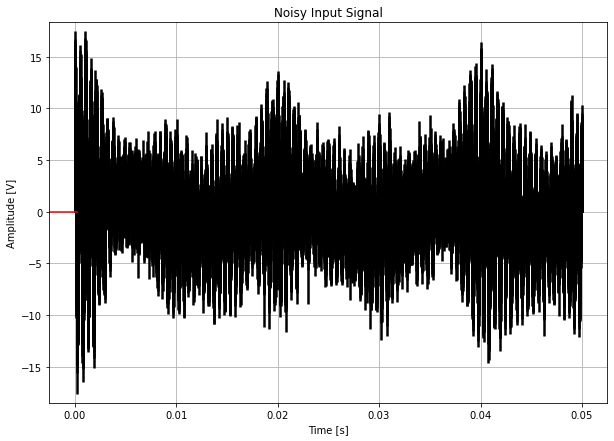
\includegraphics[scale = 0.59]{Lab 12 - Plots/Noisy Input Signal.png}\\[1.0 cm]
\end{center}

The overall magnitude information for the entire frequency range is shown next. This plot highlights the effects of the various noise factors and provides another quick check for the upcoming filter operation. It ties together the information that will be seen in the following subsections and provides context. \\ 

\begin{center}
	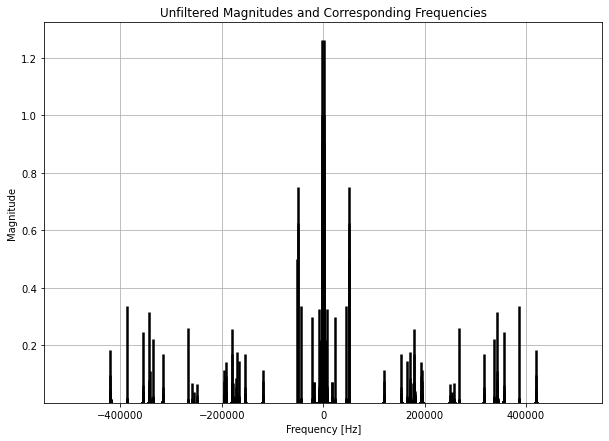
\includegraphics[scale = 0.65]{Lab 12 - Plots/Unfiltered FFT1.png}\\[1.0 cm]
\end{center}

The first magnitude intervals expressly requested in the lab were for the low frequency and switching amplifier ranges shown below. The first subplot covering the low frequencies reveals an increase in noise as it approaches the position measurement location. Likewise, the second shows noise that directly follows the passing frequency range. These regions of noise will be the most difficult to reduce given their proximity to the critical region. The plot suggests that a narrow bandpass filter would be required to attenuate these points successfully. The high noise magnitudes, on the other hand, are more likely to see reduction due to their increased distance from the center frequency, allowing even a more gradual filter slope decline to reach a reasonable attenuation. \\

\begin{center}
	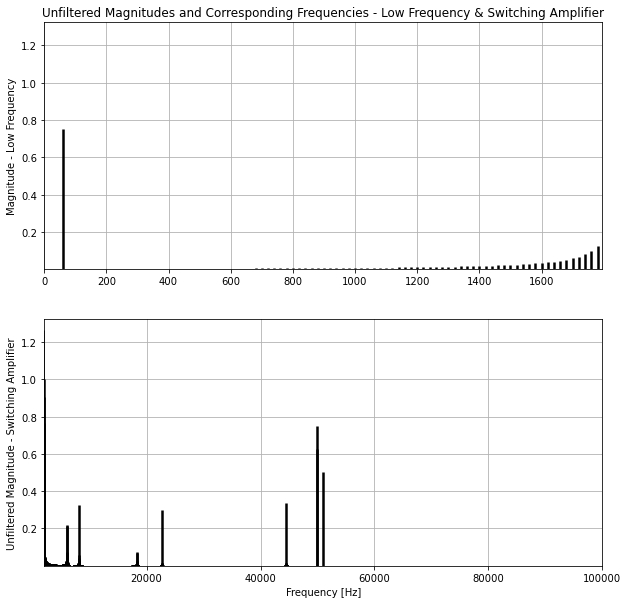
\includegraphics[scale = 0.6]{Lab 12 - Plots/Unfiltered FFT2.png}\\[1.0 cm]
\end{center}

The fast fourier transform magnitude results for the position measurement information are captured in the following plot. As with the prior plots, we can see that the proper frequency interval is being shown and matches our expectations given the overall plot. By identifying the maximum amplitude to be a little above 1.2, we can consider whether the final filtering of this region is minimally attenuated. The general sinusoidal shape of the peaks should likewise be retained. \\

\begin{center}
	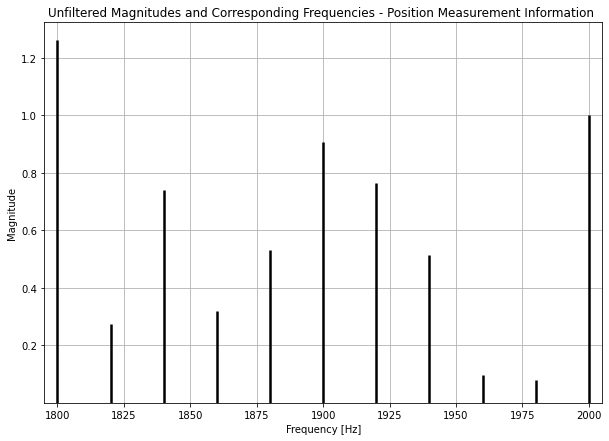
\includegraphics[scale = 0.5]{Lab 12 - Plots/Unfiltered FFT3.png}\\[1.0 cm]
\end{center}

The final fast fourier interval covering the high frequencies is plotted below. As this range should ultimately be completely attenuated with the filter active, the presence of any noise at all is the most notable feature. The desired range is properly displayed within this limited view of the x-axis and matches that of the overall magnitude plot. \\

\begin{center}
	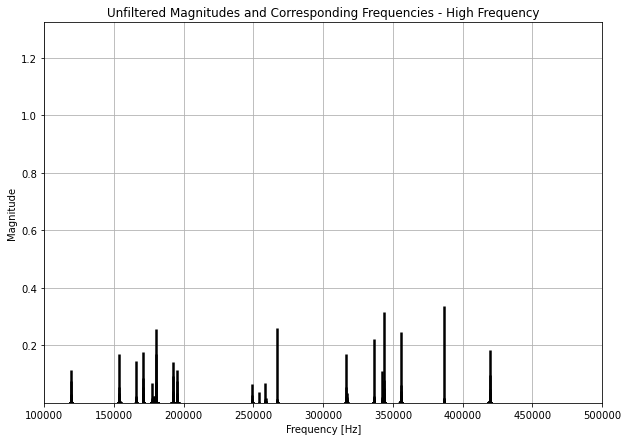
\includegraphics[scale = 0.5]{Lab 12 - Plots/Unfiltered FFT4.png}\\[1.0 cm]
\end{center}

As an RLC bandpass filter was discussed in a prior lab, this filter design was also chosen to utilize the same circuit. The transfer function given in that lab, the final component values, and the circuit schematic are shown below. \\

Transfer Function:
\begin{equation*}
	H(s) = \frac{\frac{R}{L}s}{s^2+\frac{R}{L}s+\frac{1}{LC}}
\end{equation*}

Components:
$$ R = 2.13 k\Omega, $$
$$ L = 70.3 mH, $$
$$ C = 100 nF $$

\begin{figure}[h]
	\begin{center}
		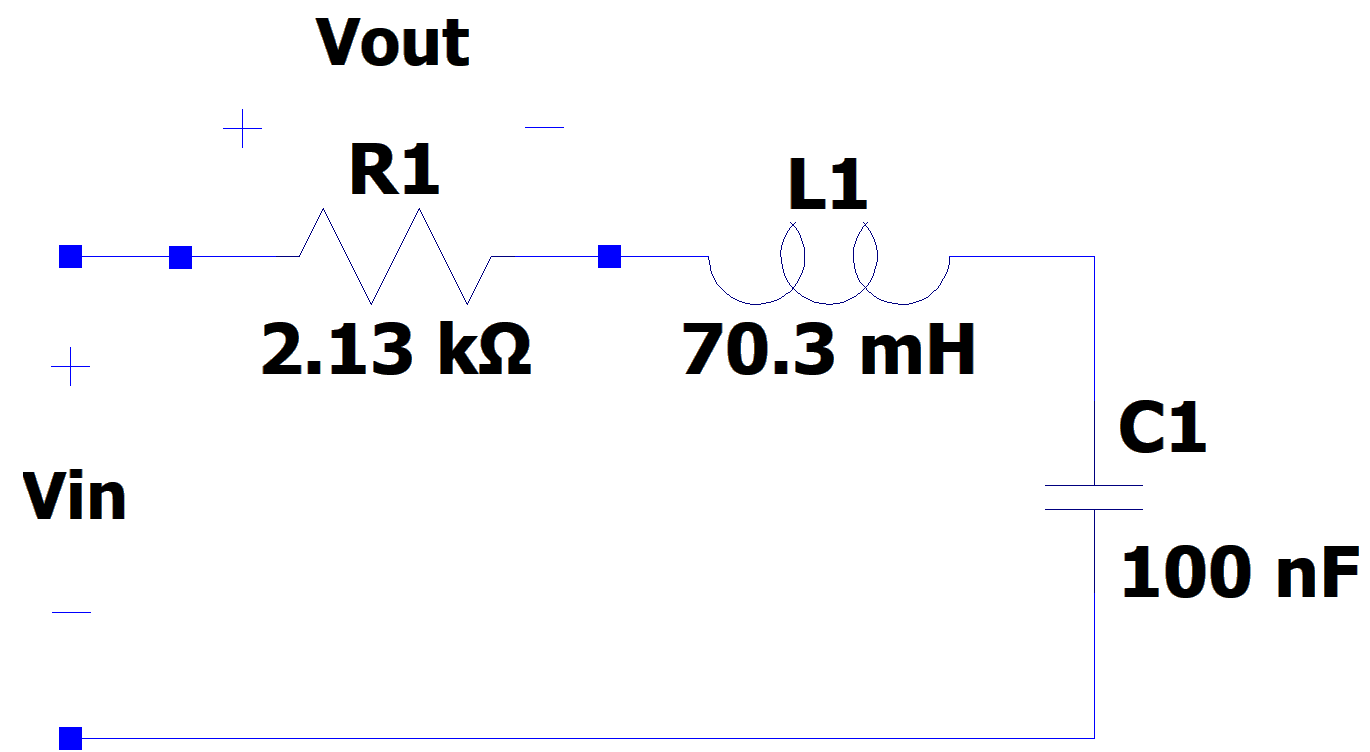
\includegraphics[scale = 0.5]{Lab 12 - Schematic/RLC Schematic.png}\\[0.01 cm]
		\caption*{\small RLC Filter Circuit Schematic}
	\end{center}
\end{figure}

The following graph shows the Bode plot for the filter design prescribed above. Despite not using the Control package to produce the plot directly, the results are identical after the necessary parameter conversions. Using this plot primarily alongside the print procedure provided in the Methodology section, the value of the resistor was altered towards the satisfaction of the filter requirements. The magnitude subplot suggests that the center frequency is properly set about midway within the position measurement range ($ 1.9\cdot10^3 $ Hz). While the peak appears sufficient to minimally attenuate this region, the lack of a steep slope for the filter reveals that the surrounding frequencies will struggle to meet their reduction criteria. \\

\begin{center}
	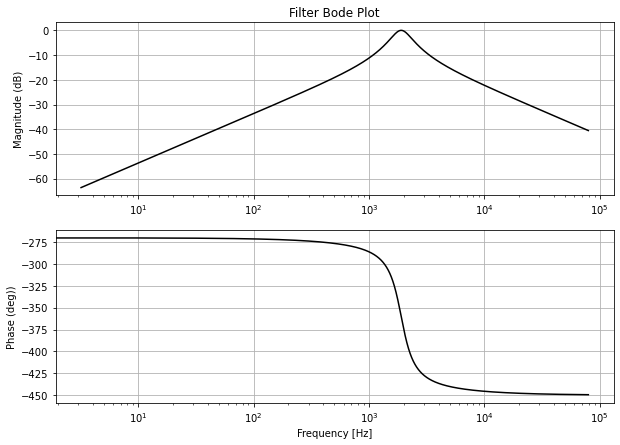
\includegraphics[scale = 0.5]{Lab 12 - Plots/Filter Bode Plot.png}\\[1.0 cm]
\end{center}

The Bode plot of the filter low frequency range indicates that its -30 dB specification for this interval is only fully met through the left portion of frequencies. The gradual -20 dB per decade slope limited by the basic RLC bandpass filter design is not sufficient to meet the attenuation goals for each interval. Either the edges of the position measurement range will see a reduction of greater than -0.3 dB, or the surrounding frequencies will not be attenuated enough. \\

\begin{center}
	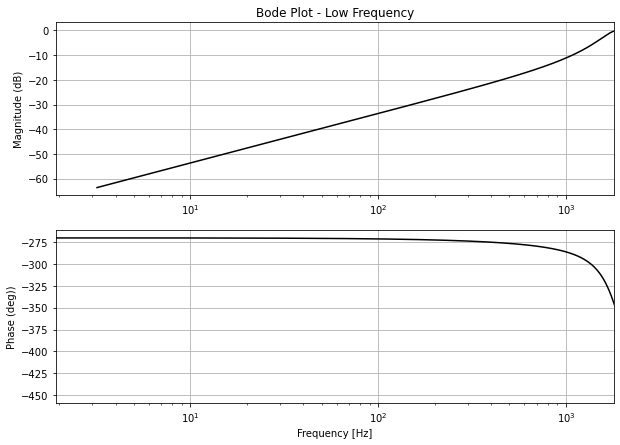
\includegraphics[scale = 0.5]{Lab 12 - Plots/Bode1.png}\\[1.0 cm]
\end{center}

The position measurement information Bode plot is given next with the interval properly defined. After adjusting the circuit component values in accordance with its effects on this range, an attenuation of less than -0.3 dB was achieved across the entire range. As this requirement was prioritized, the surrounding regions did not fully attenuate as desired. The slope could not be altered with this design. \\

\begin{center}
	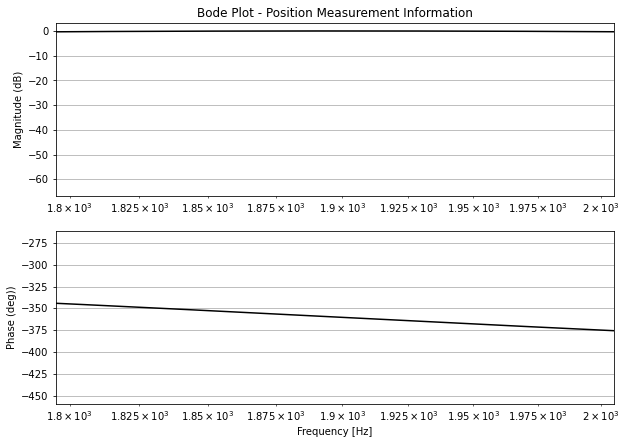
\includegraphics[scale = 0.46]{Lab 12 - Plots/Bode2.png}\\[0.5 cm]
\end{center}

The switching amplifier range Bode plot is shown below, and just as was the case for the low frequency range, the interval does not meet its attenuation goal fully. The leftmost portion does not fall below -21 dB. Again, this was due to the focus on the measurement accuracy.

\begin{center}
	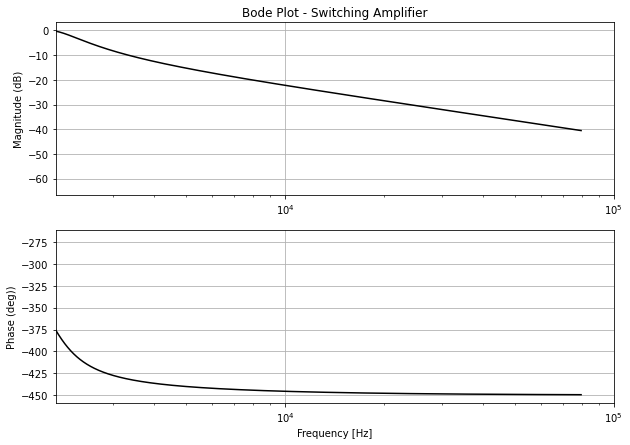
\includegraphics[scale = 0.46]{Lab 12 - Plots/Bode3.png}\\[1.0 cm]
\end{center}

The Bode plot for the high frequency range is given next. Despite the proper x-axis on display, the content of this plot is entirely blank. This matches expectations as the goal was for this region to be fully attenuated. This suggests that the filter will successfully reduce the high frequency noise. \\

\begin{center}
	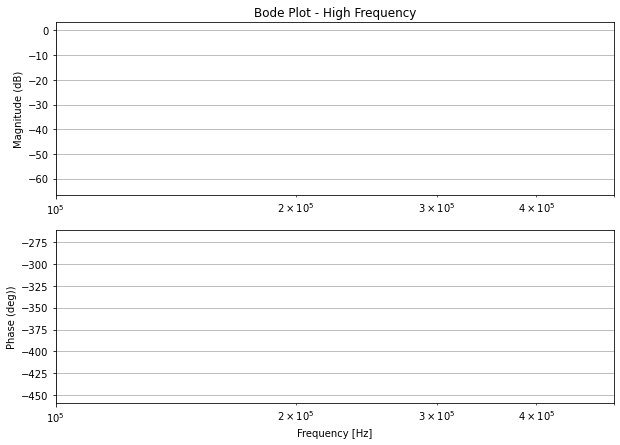
\includegraphics[scale = 0.41]{Lab 12 - Plots/Bode4.png}\\[0.5 cm]
\end{center}

Having sent the sensor signal through the filter, the resultant filtered signal is presented below. It is immediately apparent that while the x-axis has remained unchanged, the maximum amplitude is now only about 10 V as opposed to the original which was over 15 V. The signal is, however, far cleaner as can be visually verified. The overall shape has been preserved, while much of the unnecessary noise has been reduced. It is  evident that the reduction could still be improved with a more narrow bandpass filter.

\begin{center}
	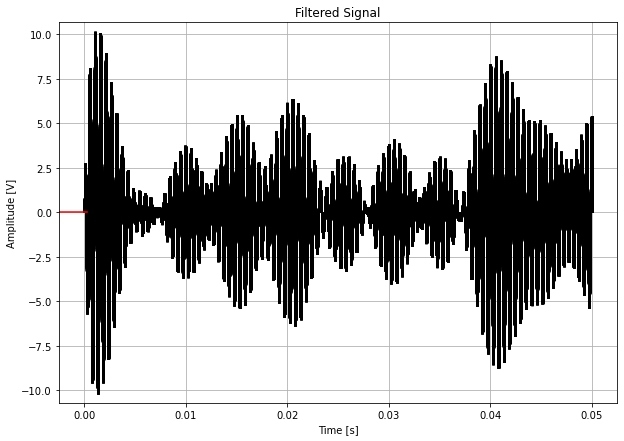
\includegraphics[scale = 0.45]{Lab 12 - Plots/Filtered Signal.png}\\[1.0 cm]
\end{center}

The filtered overall magnitude results of the fast fourier transform are shown below. The maximum magnitude which was originally a little above 1.2 has been only minimally reduced from that original plot. All of the prominent peaks apart from those surrounding the central values have been attenuated significantly. This suggests that the filter, while gradual in its slope, is still effective towards the outer extremes. \\

\begin{center}
	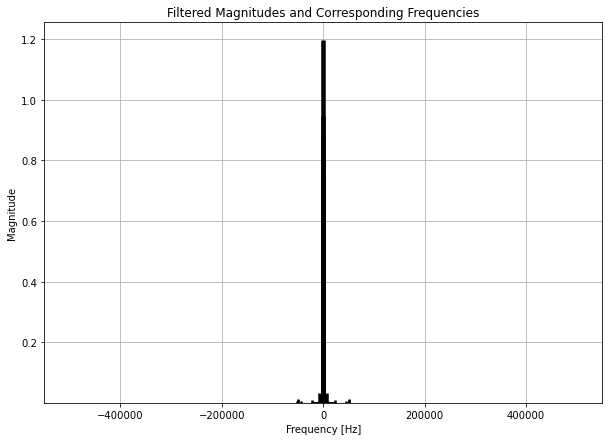
\includegraphics[scale = 0.5]{Lab 12 - Plots/Filtered FFT1.png}\\[1.0 cm]
\end{center}

The following low frequency and switching amplifier fast fourier magnitudes reinforce the conclusion that the filtering is not as effective as it should be towards the outer bounds of the position measurement range. While the other points have been attenuated, it is visually quite clear that these inner sections lack significant reduction when compared with their original counterparts. \\ 

\begin{center}
	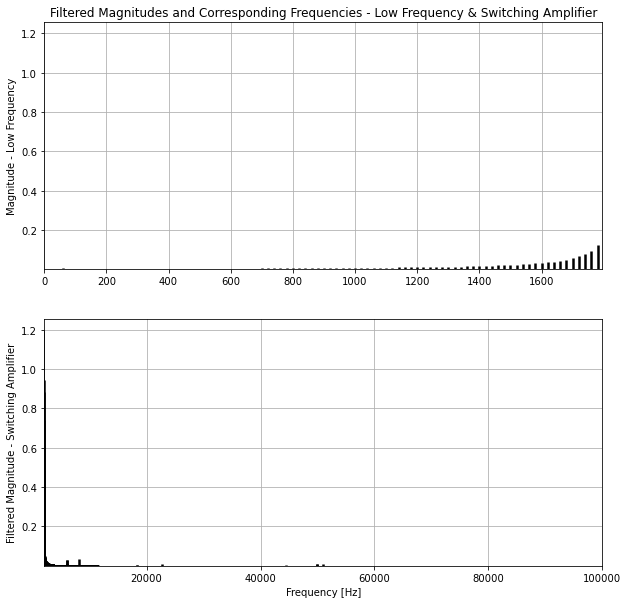
\includegraphics[scale = 0.5]{Lab 12 - Plots/Filtered FFT2.png}\\[1.0 cm]
\end{center}

The magnitude plot of the position measurement information shown below reveals that the prioritization of this region was successful in allowing the values to pass through the filter with extremely minor attenuation. The plot is nearly identical to its original counterpart, with a slight vertical decline at each point. This graph supports the viability of the filter design in its ability to properly allow a specified region to pass relatively unaltered. \\

\begin{center}
	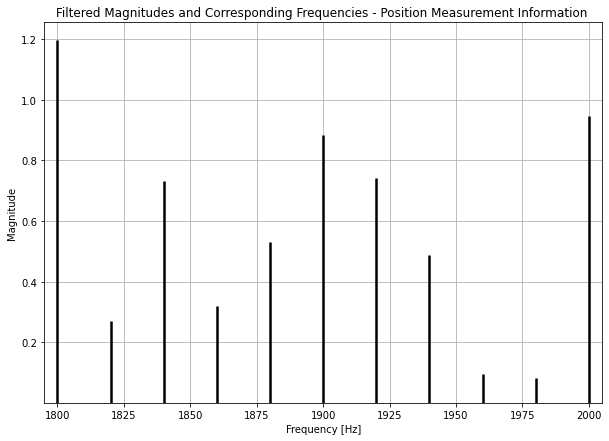
\includegraphics[scale = 0.5]{Lab 12 - Plots/Filtered FFT3.png}\\[1.0 cm]
\end{center}

The final plot shows the high frequency fast fourier result for the filtered signal. There are no magnitudes represented on the graph, indicating that the original noise has been altogether attenuated. Consequently, the filter design appears to be successful in achieving the goal for this region of the input signal. \\

\begin{center}
	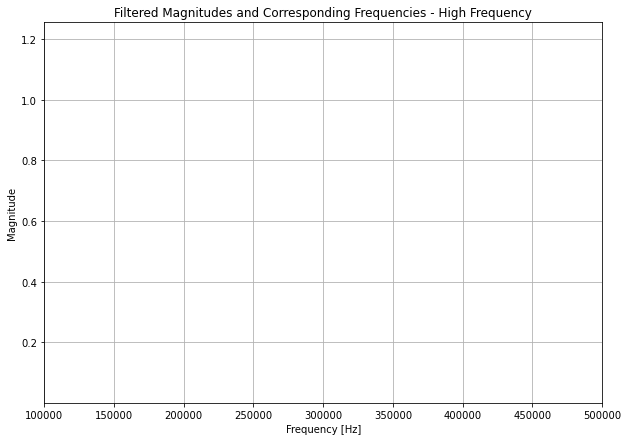
\includegraphics[scale = 0.5]{Lab 12 - Plots/Filtered FFT4.png}\\[1.0 cm]
\end{center}

\section{Error Analysis}

I was unable to design a filter that properly attenuated the low frequency by -30 dB and the switching amplifier range by -21 dB across the entire intervals. The reason for this problem is due to the type of circuit used and its resultant transfer function. The RLC bandpass filter has a transfer function that does not allow for steep slopes. The inductor and capacitor influence the position of the center frequency, while the resistor impacts the bandwidth. Consequently, the resistor is the only component that should be adjusted. \\

In order establish the pass frequency range, the slope is necessarily gradual such that the attenuation of the points surrounding the bounds of the range is less successful. The value of the resistor can be increased to such a degree that the sort of attenuation required for the other frequency ranges is attainable, but the trade-off is that the outer values of the position measurement interval would see high attenuation. I was not able to resolve this issue using the RLC circuit design, and prioritized the minimal attenuation of the pass frequency region. \\

\section{Questions}

When asked what I personally wanted to get out of taking this course, I responded: ``I would like to better understand the material presented in the lectures,
improve my skills in Python, and learn to use LaTeX." I feel that all of these goals were met. This lab certainly improved my understanding of class material, particularly in understanding the basis of many concepts and the general idea of convolution. I learned many new functions in Python and learned more of the syntax. I also feel quite comfortable working in LaTeX now and have come to appreciate it. \\

\section{Conclusion}

This lab presented a real-world problem involving filters that required close consideration of the material covered in this course. The process helped solidify the information while challenging our ability to solve problems independently. It required that we understand our errors, determine the cause behind the issue, and explain our findings. It also pushed us to write professional lab reports that are both comprehensive and cohesive. \\

Although I struggled with this lab and did not satisfactorily meet all expectations, I do not think that the lab needs any changes. The level of challenge is right were it needs to be and the independence pushes us to review and contemplate. The careful consideration of a problem statement and review of old material required by this lab will be of use in the future. Grappling with practical problems will improve our long-term understanding of these concepts. \\

\newpage
\begin{thebibliography}{111}
	
	\bibitem{S}
	Sullivan, Dennis M. (2018) {\it  Signals and Systems for Electrical Engineers I}. Nevada: CreateSpace Independent Publishing Platform.
	
\end{thebibliography}
\end{document}

% Lab Report based on template created by Roza Aceska.